\subsection{Kalibrierung der großen Scheibe}
Mit der großen Scheibe funktioniert die Bestimmung der Winkelrichtgröße $D$ genauso wie für die kleine Scheibe mit der Ausnahme, dass hier direkt der Drehmoment und der Winkel in $[\mathrm{rad}]$ angegeben wurde, sodass sich die Winkelrichtgröße direkt aus der Steigung ablesen lässt. Aus diesem Grund werden hier nur die Werte (inkl. Fehler) angegeben. Es ergibt sich über die Methode der statischen Kalibrierung folgender Wert (Daten, siehe Abb. \ref{fig:kal3})
\begin{align*}
D = \unit[(2.17 \pm 0.04)]{N m}
\end{align*}
Die großen Fehlerwerte ergeben sich dadurch, dass die rücktreibende Kraft von der Richtung, in die die Scheibe ausgelenkt wird abhängt (materialbedingt).

\begin{figure}
\begin{center}
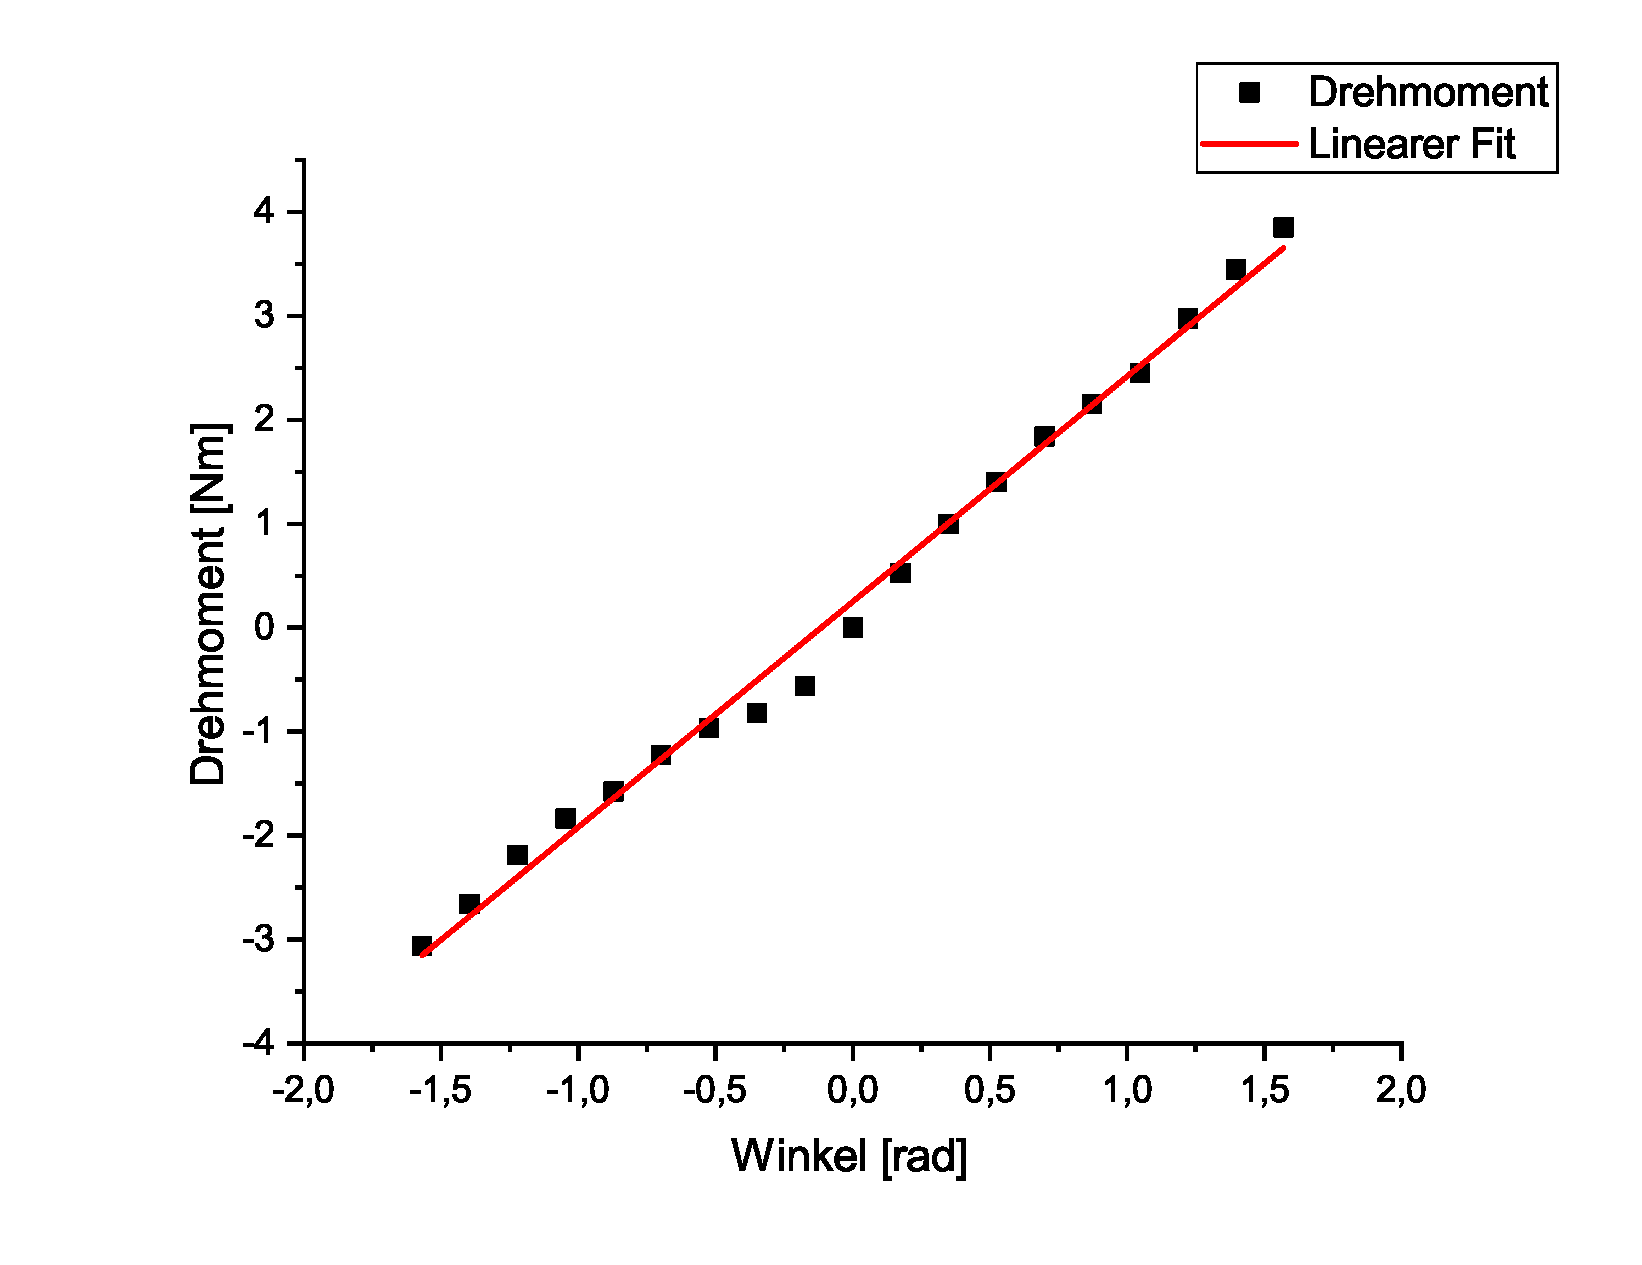
\includegraphics[width=0.7\textwidth]{Bilder/kal3.eps}
\caption{Statische Ermittlung der Winkelrichtgröße von der großen Scheibe}
\label{fig:kal3}
\end{center}
\end{figure}

Zudem ist das Material sowie die Abmessungen der Scheibe bekannt, also kann der Trägheitmoment berechnet werden:
\begin{equation}
J_0 = \frac{1}{2} m \cdot r^2 = \frac{1}{2} d\cdot r^2 \cdot \rho \pi r^2 = \unit[0.67]{kg m^2}
\end{equation}
Also kann die Winkelrichtgröße $D$ auch mithilfe von der gemessenen Zeit sowie Formel \ref{eq:wink} $D = \unit[(2.27 \pm 0.3)]{N m}$.\\
Dieser relativ große Fehler ergibt sich durch die Ungenauigkeit im Radius, der mit der vierten Potenz in die Rechnung eingeht.






